%\begin{tcolorbox}[breakable,colback=black!5!white,colframe=red!80!black,width=\textwidth]
\chapter{The Large Hadron Collider and the CMS experiment}
%\end{tcolorbox}
\label{chap:LHC_CMS}
Brief intro to CERN and LHC
\begin{itemize}
\item research
\item technology
\item education
\item collaboration
\end{itemize}

\section{The Large Hadron Collider}
The Large Hadron Collider (LHC) is a 27 km ring structure designed for the acceleartion and collision of protons and heavy ions. It is situated approximatively 100 m underground, between France and Switzerland, in the Geneva area, and it is the most important of the CERN (Conseil europ\'een pour la recherche nucl\'eaire) facilities. In order to reduce the cost of the project, definetively approved in 1996, the LHC has been designed to fit the pre-existing underground tunnel of the Large Electron-Positron collider (LEP) [ref. 24 Jacopo], built to accelerate electrons and positrons and running until the year 2000.\\
Moving from an electron-positron collider to an hadron collider allowed to reach higher energies in the center-of-mass frame, since the syncrotron radiation loss is inversely proportional to the fourth power of the mass of the particle involved: hence, it is reduced by a factor $m_p/m_e \sim 10^3$. Furthermore, at a proton-proton collider it is possible to collect higher luminosities (and hence more statistics) with regards to, for example, a proton-antiproton collider, like Tevatron at Fermilab, in the USA.\\
In the LHC two identical beam pipes rings are designed to let protons circulate in opposite directions, in ultrahigh vacuum conditions ($10^{-11}$--$10^{-10}$ mbar) in order to avoid collisions with gas molecules. Given the reduced available diameter in the tunnel (4 m), the two proton beams are magnetically coupled. The collider is composed by 8 arc sections (48 km) driving protons around the ring, and straight sections (6 km) where beam control systems and detectors are inserted. Proton beams collide in four interaction points, where the four main LHC experiments are installed: ALICE, ATLAS, CMS, LHCb.

\begin{figure}[!htb]
  \centering
    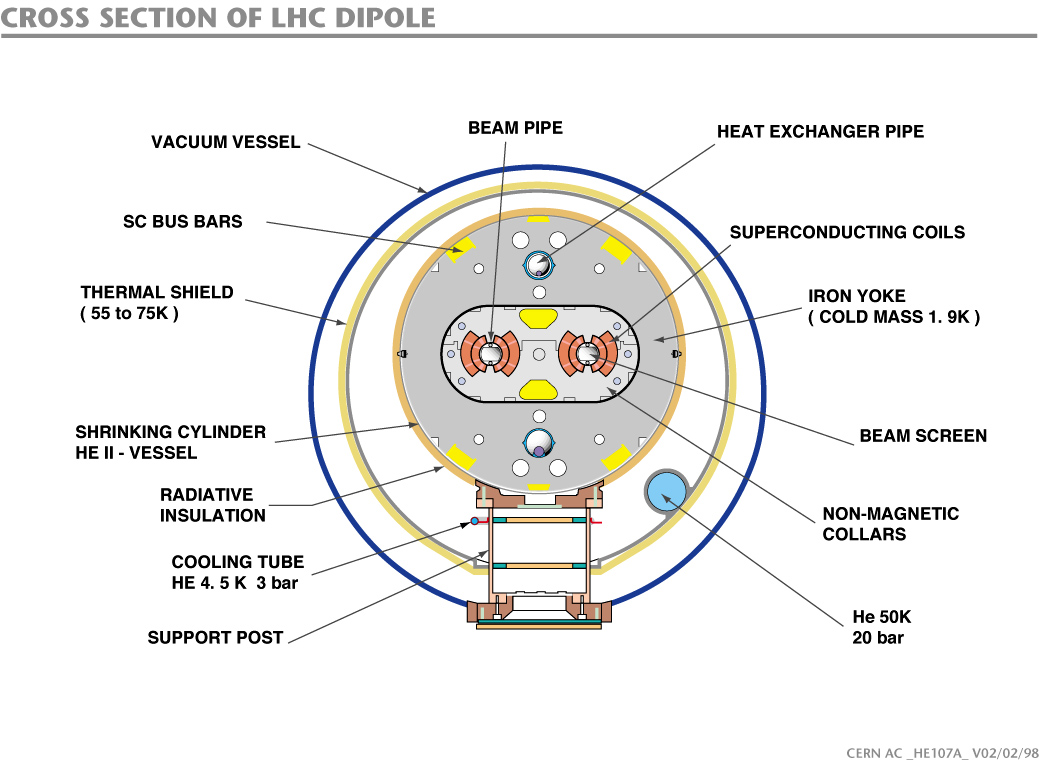
\includegraphics[width=.6\textwidth]{figures/LHC-magnets.jpg}
  \caption{Section of the LHC dipole magnet structure.}
  \label{fig:LHC_dipole}
\end{figure}

\noindent In fig.~\ref{fig:LHC_dipole}, a slice of the arc section is displayed. Around the beam pipes, two superconducting magnetic dipoles are located: they generate vertical magnetic fields in opposite directions. The superconducting coils are made of niobium-titanium, materials that are superconducting at very low temperature. At the LHC, they are kept at a temperature of 1.9 K (-$271.3^{\circ}$C) by a closed liquid helium circuit. A current of 11850 A flows through the magnets, without any energy loss due to electrical resistance, generating a magnetic field of 8.33 T. Magnets of higher order in multipole expansion (quadrupoles, sextupoles, octupoles, ...) are used to optimize the proton trajectories; in particular, quadrupoles allow to focus and squeeze the beams. Along the LHC ring here are 9593 magnets; 1232 are dipoles, 392 are quadrupoles.

\begin{figure}[!htb]
  \centering
    %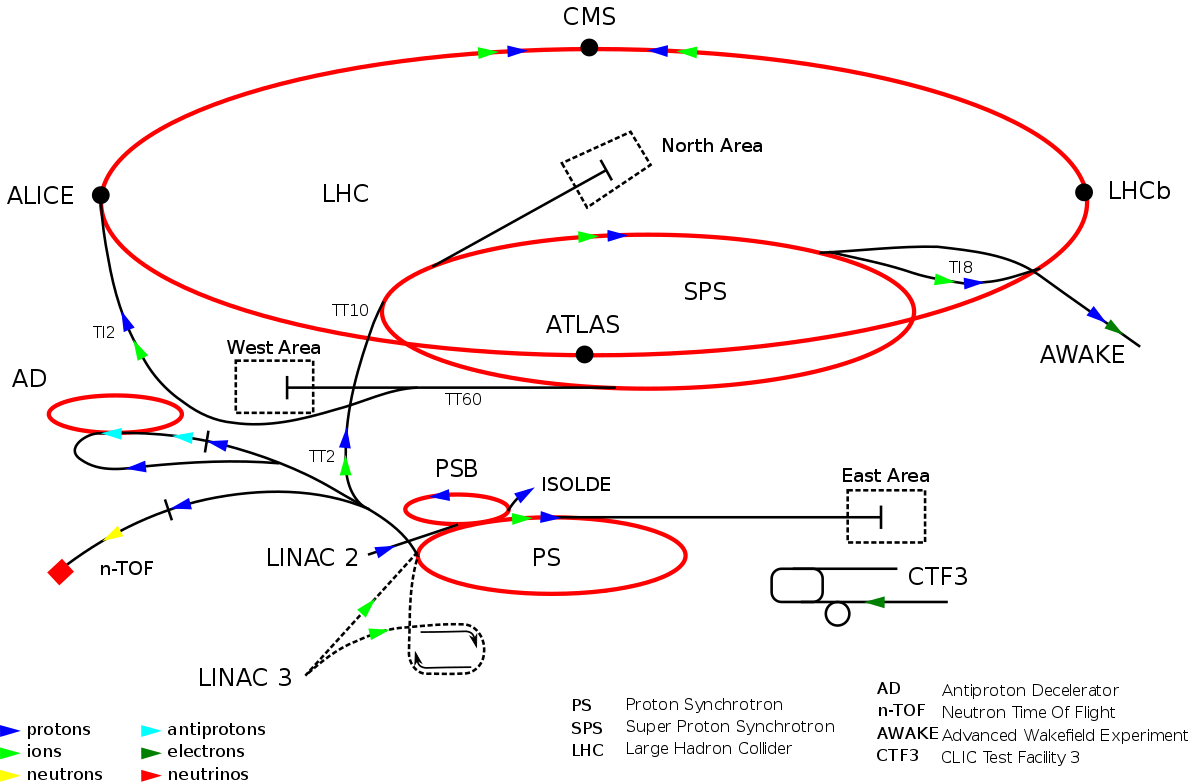
\includegraphics[width=.75\textwidth]{figures/Cern-accelerator-complex.png}\\
    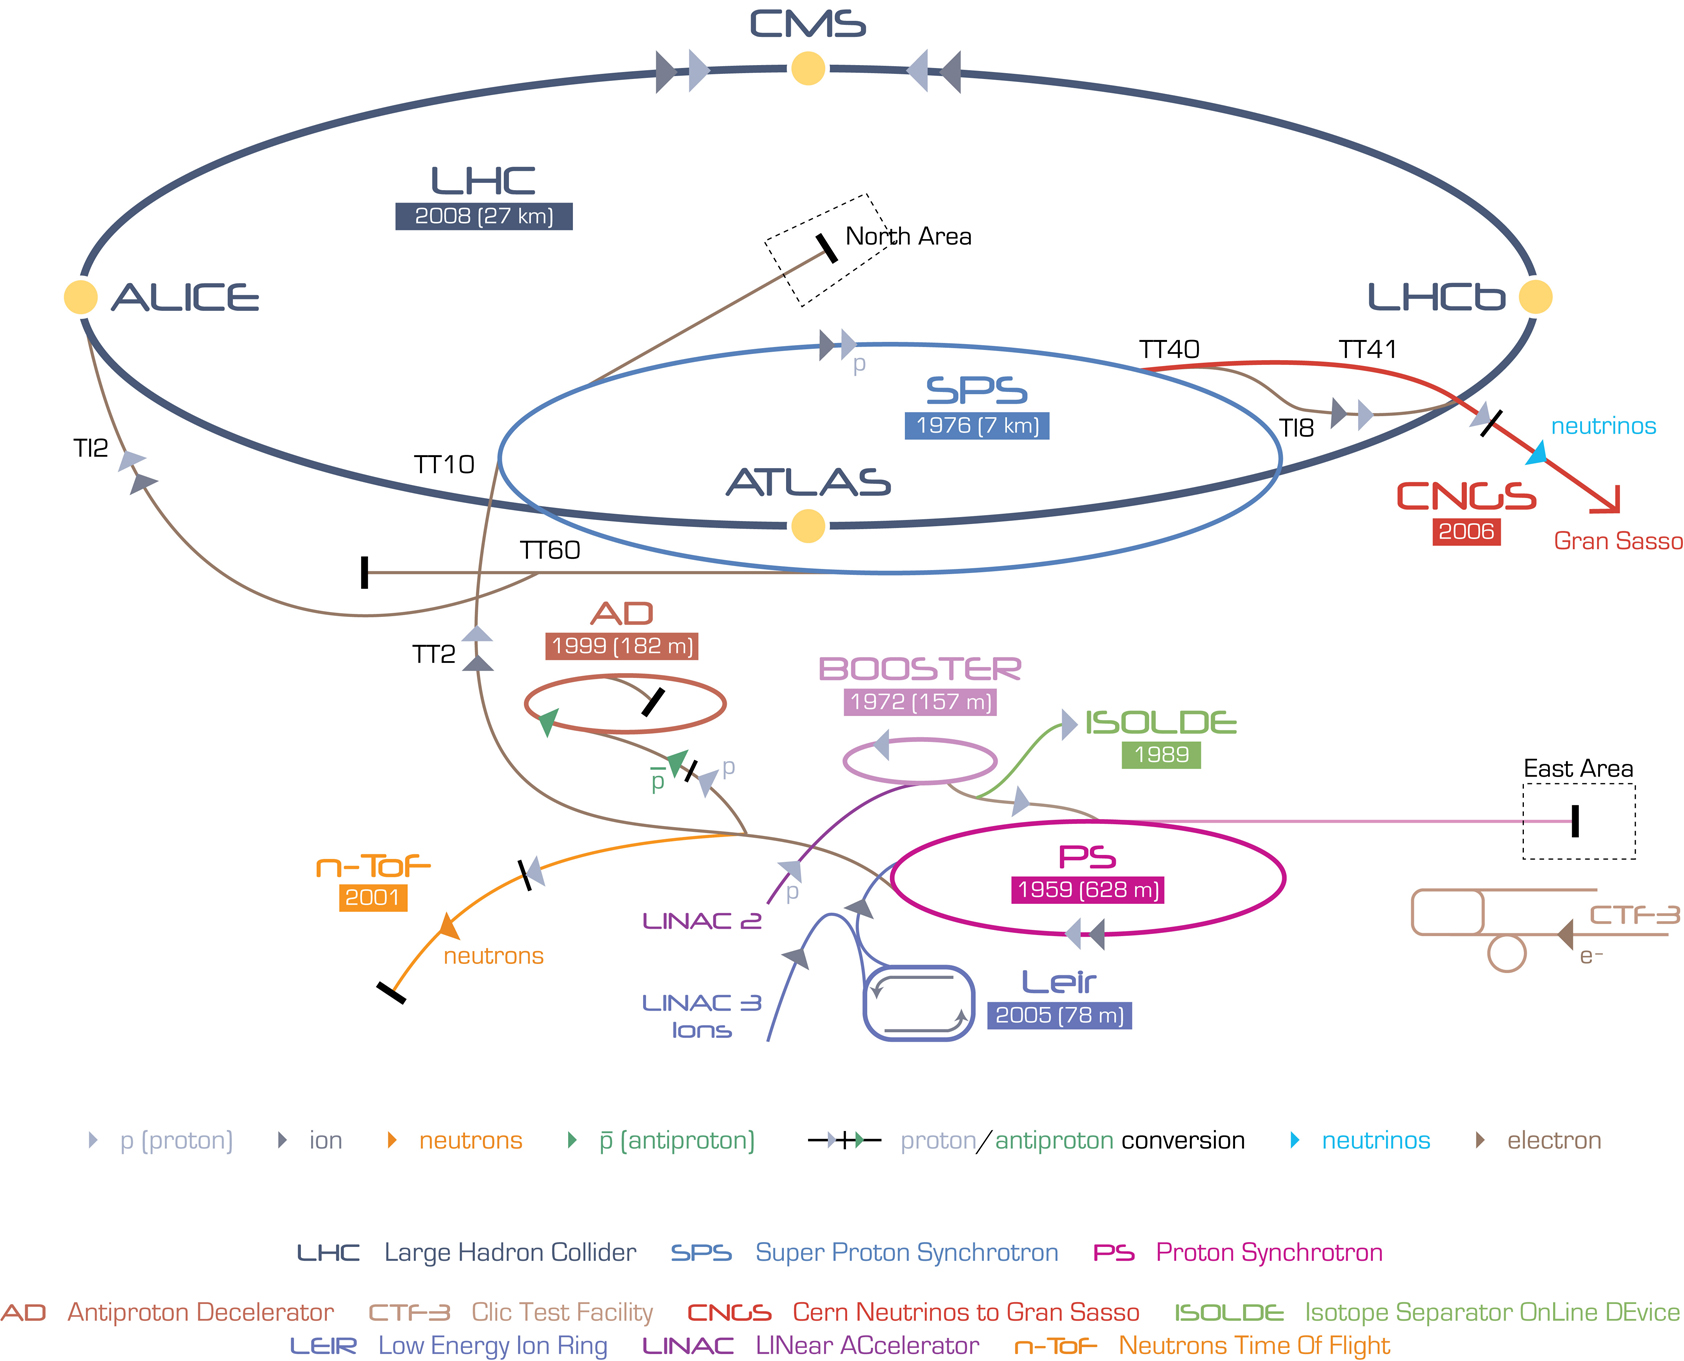
\includegraphics[width=.75\textwidth]{figures/Cern-Accelerator-Complex.jpg}
  \caption{The CERN accelerator complex.}
  \label{fig:LHC_accelerator_complex}
\end{figure}

\noindent The LHC represents the final step of the CERN accelerator complex, showed in fig.~\ref{fig:LHC_accelerator_complex}. Protons are extracted from hydrogen atoms and inserted in the linear accelerator Linac2, that brings them to an energy of 50 MeV. They circulate around a little synchrotron, Proton Synchrotron Booster, reaching an energy of 1.4 GeV, and then in the Proton Syncrhrotron (PS), where their energy is increased to 25 GeV. The second to last step is the Super Proton Synchrtotron, SPS, accelerating protons up to 450 GeV. They are finally injected in the Large Hadron Collider, where sixteen radiofrequency cavities (RF) accelerate protons inside each beam up to an energy of 6.5 TeV, providing a center-of-mass energy of 13 TeV when colliding. The RF cavities provide an accelerating electromagnetic field up to 5 MV/m (maximum voltage of 2 MV), that oscillates with a frequency of 400 MHz. Like the magnets, the cavities are kept at low temperature (4.5 K, or -$268.7^{\circ}$C) in order to allow superconducting conditions. The maximum beam energy can be reached in 15 minutes. After several hours of collisions ($\sim$ 10 hours), the quality of the beams deteriorates and they are extracted from the machine and dumped.\\

\noindent Protons circulate inside the LHC ring in bunches of $\sim10^{11}$ particles each, 80 mm long. Focusing magnets allow to reduce the bunch diameter down to 16 $\mu$m. Different bunches are separated by 25 ns (or, $\sim 7.5$ m), corresponding to a frequency of 40 MHz and an instantaneous (peak) luminosity (defined in eq.~\ref{eq:LHC_luminosity_def}) of $1.2 \times 10^{34}\mbox{ cm}^{-2} \mbox{s}^{-1}$. Given the structure of the beams, at every bunch crossing many protons interact simultaneously: this phenomenon is called pile-up. The designed maximum number of bunches is 2808.\\
%Protons with slightly different energies arriving earlier or later will be accelerated or decelerated so that they stay close to the energy of the ideal particle. In this way, the particle beam is sorted into discrete packets called "bunches". Top energy is reached in around 15 minutes, the bunches having passed the cavities around 1 million times.
%Queste frequenze elevate generano un problema noto con il nome di ``pile-up'', che consiste nel moltiplicarsi del numero di vertici primari di interazione. Ad un medesimo evento registrato prodotto dalle collisioni ogni 50 ns, infatti, corrispondono fino a 30 vertici di interazione; essi aumenteranno a 40 quando si arriver\`a a realizzare una collisione ogni 25 ns.\\

\begin{figure}[!htb]
  \centering
    \includegraphics[width=.5\textwidth]{PPD_results/int_lumi_per_day_cumulative_pp_2016.pdf}%
    \includegraphics[width=.5\textwidth]{PPD_results/int_lumi_per_day_cumulative_pp_2016_Golden_23Sep-PromEraH_Morion.png}

    \includegraphics[width=.5\textwidth]{PPD_results/int_lumi_per_day_pp_2016.pdf}%
    \includegraphics[width=.5\textwidth]{PPD_results/pileup_pp_2016.pdf}

  \caption{Luminosity in 2016 LHC data. Top-left plot: the cumulative integrated luminosity delivered by LHC (in blue) and recorded by CMS (in orange), as a function of the data taken period. Top-right plot: data recorded by CMS and declared as optimal for the physics analyses (in light orange), corresponding to a total integrated luminosity of 35.9 $\text{fb}^{-1}$. Bottom-left plot: maximum integrated luminosity per day. Bottom-right plot: number of proton interactions per bunch crossing (pile-up).}
  \label{fig:LHC_lumi}
\end{figure}

\noindent The main parameters that describes an hadronic collider are the center-of-mass energy, corresponding to the sum of the energies of the beams, and the instantaneous luminosity, that describes the frequency of the interactions among the bunches in the beams. If the bunches in the first beam contain $n_1$ protons, and the bunches in the second beam contain $n_2$ protons, and if the colliding area is $\Sigma$, the frequency of complete turns
around the ring is $f$, the instantaneous luminosity $\mathcal{L_{\text{inst}}}$ is:

\begin{equation}
\mathcal{L_{\text{inst}}} = f \frac{n_1 n_2}{\Sigma}.
\label{eq:LHC_luminosity_def}
\end{equation}

\noindent If a generic physics procces $i$ has a cross-section of $\sigma_i$, the interaction rate $R_i$ is:
\begin{equation}
R_i = \frac{dN_i}{dt}= \sigma_i \mathcal{L_{\text{inst}}},
\label{eq:LHC_interaction_rate}
\end{equation}
and the number of events recorded in the time interval $(0,\tau)$ is obtained by the integrated luminosity $\mathcal{L} = \int_0^{\tau} \mathcal{L_{\text{inst}}} dt$:
\begin{equation}
N_i = \sigma_i \int_0^{\tau} \mathcal{L_{\text{inst}}} dt.
\end{equation}

\noindent In fig.~\ref{fig:LHC_lumi}, a summary of the luminosity measurement in 2016 data is presented. The luminosity delivered by LHC is represented in blue, the recorded by CMS is in orange. The mean number of interaction per bunch crossing (pile-up) is presented as well. The average number of interactions per collision is 27, the maximum is around 50.

\subsection{Proton-proton interactions}
\begin{figure}[!htb]
  \centering
    \includegraphics[width=.5\textwidth]{figures/78events_PU.png}
  \caption{78 events.}
  \label{fig:pp_pileup}
\end{figure}
%Figura da CMS Collaboration, DAQ generic figures gallery online at http://cmsdoc.cern.ch/cms/TDR/DAQ/TDRweb/daqgenericjpg.htm
Proton-proton collisions allow to reach higher energies and luminosities, but the drawback is the complexity of the events when compared to electron-positron collisions: not only because of the increasing backgrounds due to strong interactions among partons, but also because the momenta of the proton partons taking part in the interaction are unknown; not to mention the problem of disentangling the tracks of the particles coming from the interesting hard interactions from the spectator pile-up interactions (in fig.~\ref{fig:pp_pileup}, 78 proton collisions were happening at the same bunch crossing).\\
The majority of the LHC events is represented by soft interactions, with low transverse momentum transfer, namely elastic and diffractive scatterings. In the so-called hard interactions, on the other hand, the transferred momentum among particles is high, allowing to produce massive resonant phenomena. These events manifest in peculiar final state signatures that can be distinguished from the soft interaction background.\\
At high momentum transfer (perturbative regime), a proton can be described as a collection of partons, each bringing a fraction $x$ of the initial beam momentum, whose distribution is described by the parton distribution functions (PDF), $f(x,Q^2)$, as a function of the Bjorken's variable and of the momentum transfer $Q^2$. At very high center-of-mass energies (13 TeV), the proton masses can be neglected; the available energy in the parton 1 and parton 2 scattering is unknown, $\sqrt{x_1 x_2 s}$. The total cross-section is given by:
\begin{equation}
\sigma = \int dx_1 f_1(x_1,Q^2) \int dx_2 f_2(x_2,Q^2) \sigma_{12}(x_1 p_1, x_2 p_2, Q^2),
\end{equation}
where $\sigma_{12}$ is the cross-section at parton level, and $f_1,f_2$ are the parton PDFs. In fig.~\ref{fig:LHC_pp_cross_section}, parton cross-sections are displayed as a function of the center-of-mass energy.

\begin{figure}[!htb]
  \centering
    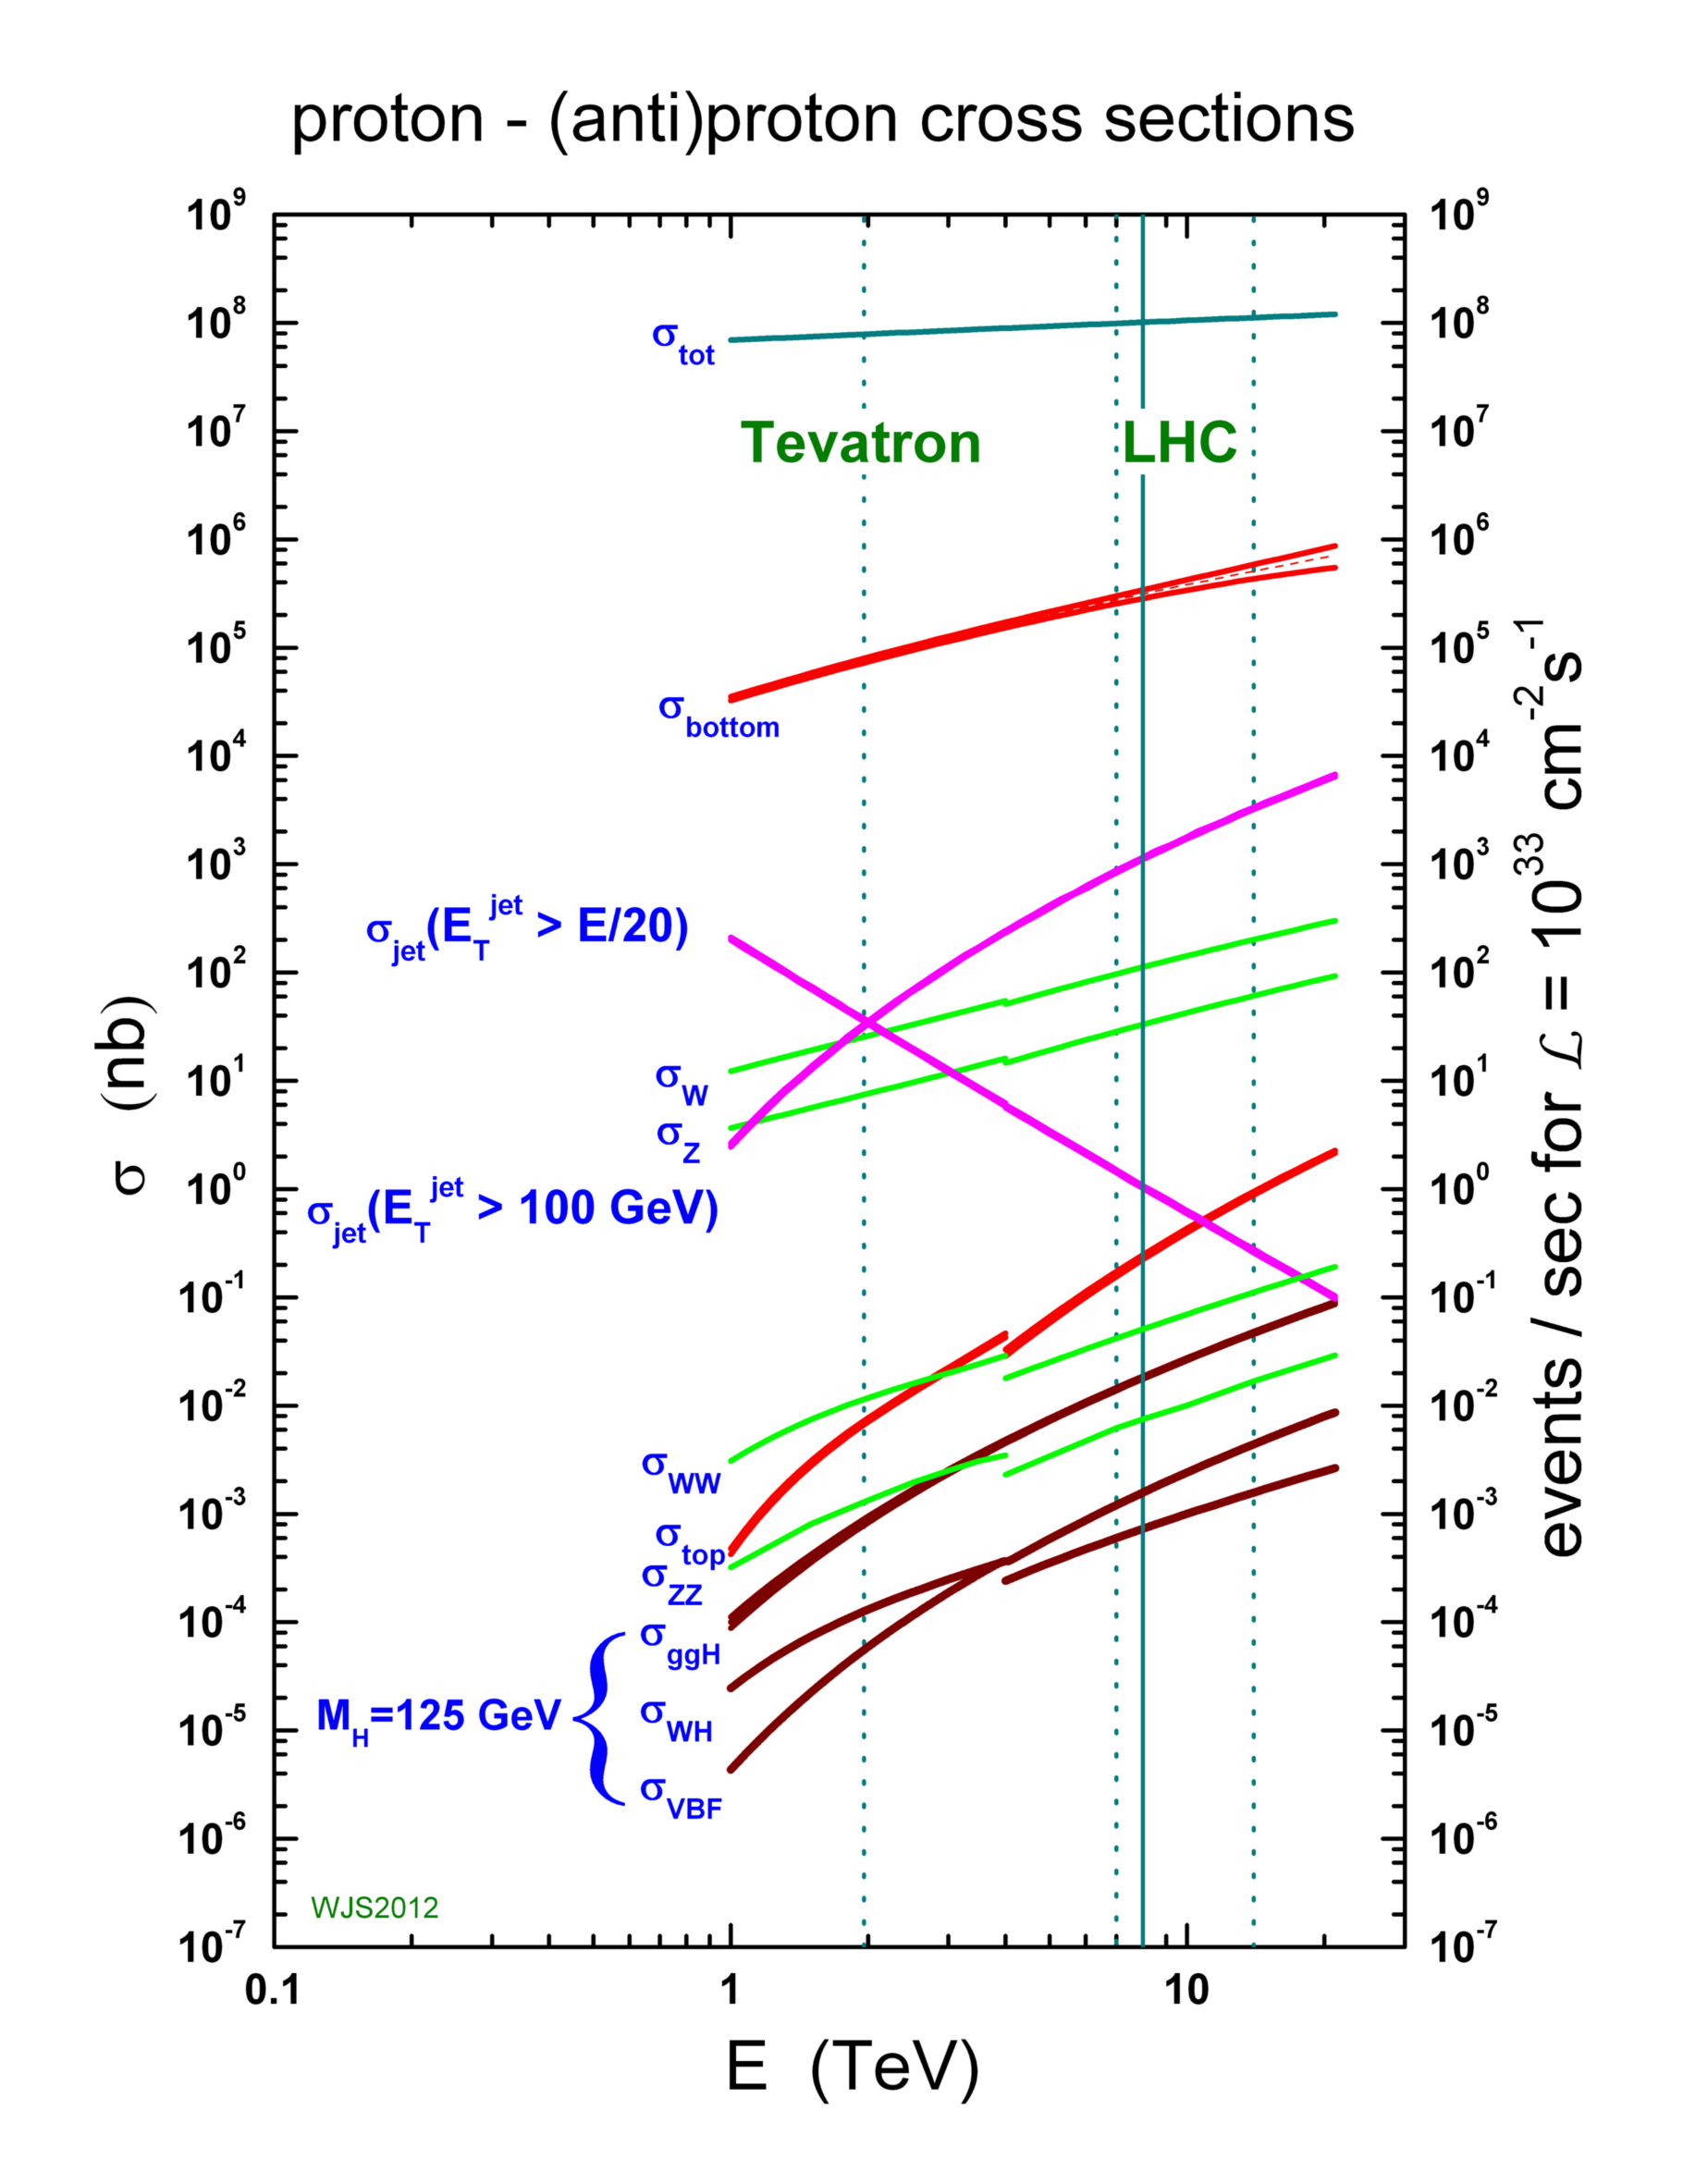
\includegraphics[width=.5\textwidth]{figures/crosssections2013.jpg}
  \caption{Cross-sections and number of expected events in proton-proton collisions, as a function of the center-of-mass energy. Rare phenomena, such as the Higgs boson production, can be observed at the LHC.}
  \label{fig:LHC_pp_cross_section}
\end{figure}

\section{CMS detector}

The Compact Muon Solenoid (CMS) is a multi-purpose detector built in the LHC ring. It is situated in a cavern 100 m underground, near Cessy, in France. It is a cylinder 22 m long, with a diameter of 15 m, and a weight of 12500 tons. Its physics programme includes the search for the Higgs boson (discovered in 2012), precision measurements of the Standard Model parameters and rare decays (physics of beauty quark), and search for new physics beyond the standard model (SUSY, exotic phenomena, dark matter, extra dimensions).\\
The CMS detector is structured in many layers of sub-detectors, giving different responses depending on the nature and the momentum of the particle passing through. The inner detectors have been finely segmented in order to afford the high radiation levels and particle multiplicity at the interaction point, so that the reduced occupancy of each layer allows to measure and distinguish precisely the primary vertices of the hard interactions from the pile-up events. A very precise time resolution is vital in order to synchronize all the subsystems together.\\
%La maggior parte dei processi fisici che si vogliono esplorare hanno basse sezioni d'urto, mentre, come \`e ben noto, i prodotti delle collisioni tra protoni sono dominati da elevati fondi QCD: CMS \`e progettato in modo da avere un'elevata capacit\`a di discriminazione degli eventi rari, sfruttando in particolare i canali comprendenti elettroni e muoni, e una grande precisione di misura dei vertici secondari, necessaria per distinguere i $\tau$ e gli adroni contenenti quark pesanti. L'elevata luminosit\`a nominale di LHC, come accennato, comporta il problema del pile-up: questi effetti possono essere ridotti utilizzando rivelatori ad elevata granularit\`a. L'occupazione si abbassa segmentando l'apparato in molti sottogruppi di rivelatori, al costo di dover ottenere un'ottima sincronizzazione tra di essi. L'alta frequenza di interazione, inoltre, necessita un'alta risoluzione temporale. Infine, gli elevati livelli di radiazione attorno al vertice richiedono apparati robusti e resistenti.

\begin{figure}[!htb]
  \centering
    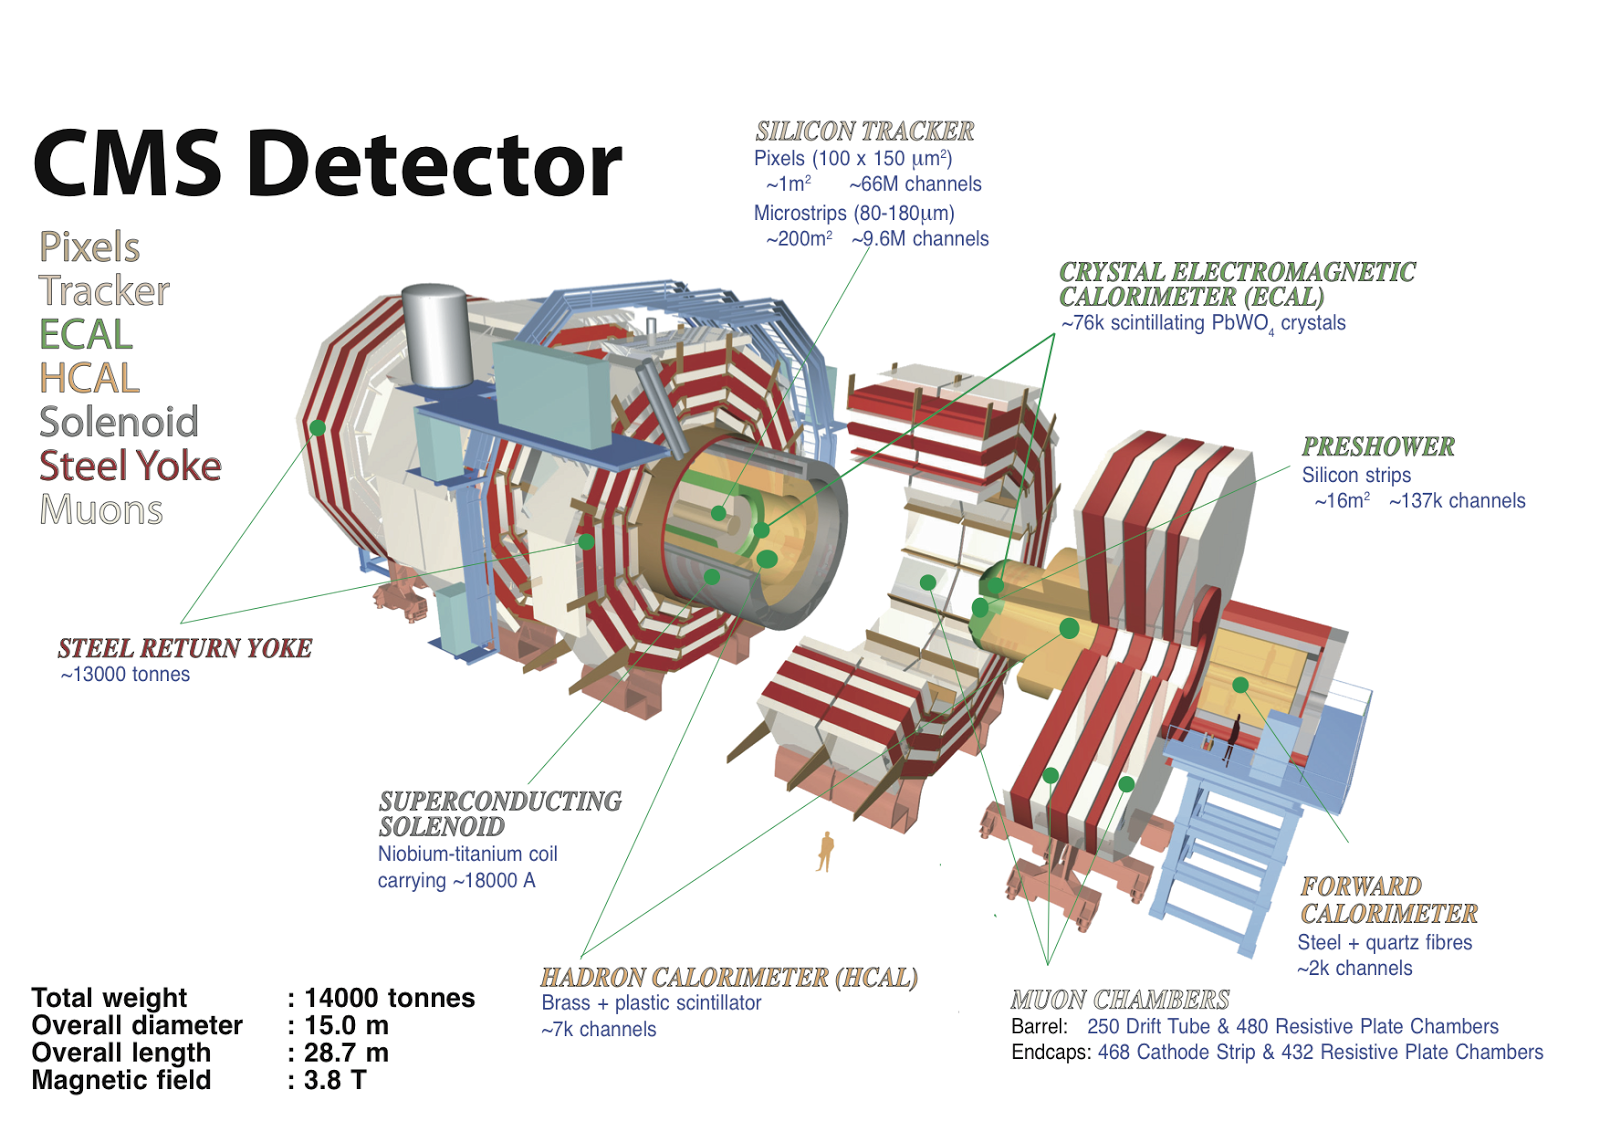
\includegraphics[width=.99\textwidth]{figures/cms_3d.png}
  \caption{The CMS experiment.}
  \label{fig:CMS_1}
\end{figure}

\noindent Fig.~\ref{fig:CMS_1} shows a sketch of the CMS detector. It is longitudinally segmented in the barrel region and two endcaps. In the forward region (over the endcaps), where the beam radiation is very intense, additional calorimeters have been placed. In fig.~\ref{fig:CMS_particles}, the mean path of a specific particle through the sub-detectors is represented, depending on its flavour.

\begin{figure}[!htb]
  \centering
    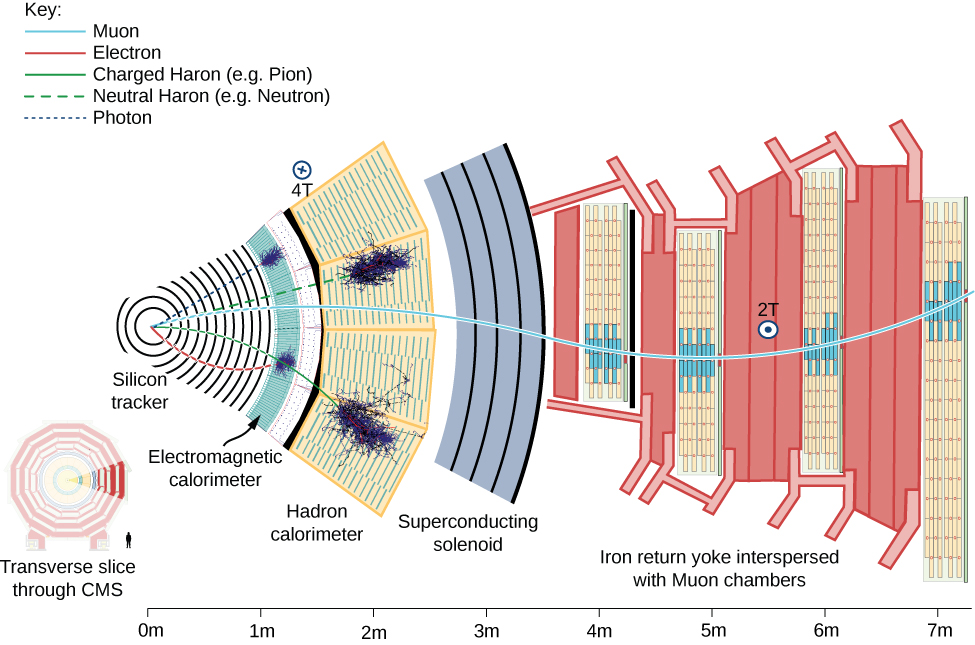
\includegraphics[width=.99\textwidth]{figures/CMS_particles.jpg}
  \caption{Mean path of a particle through the CMS detector. A muon, in light blue, passes through with a bended trajectory, depending on its momentum and charge, triggering signals in all the sub-systems. An electron, in red, leaves a track in the silicon tracker and is absorbed by the electromagnetic calorimeter. A neutral or charged hadron, in green, stops inside the hadronic calorimeter. A photon, dotted blue line, showers in the electromagnetic calorimeter, without leaving any track in the silicon detector.}
  \label{fig:CMS_particles}
\end{figure}

\subsection{The coordinate system}
The CMS cooridnate system is depicted in fig.~\ref{fig:CMS_CoordSys}. $x$ and $y$ are the coordinates in the transverse plane, $z$ is the longitudinal coordinate. The $x$ axis points at the center of the LHC ring, the $y$ axis points upward, the $z$ axis is along the beam direction. The azimuthal angle $\phi$ lays in the in the transverse plane, and it is measured starting from the $x$ axis; the radial coordinate is $r$. The polar angle $\theta$ lays in the plane $rz$. The transverse component of the 3-momentum, $\vec{p}_T$, is orthogonal to the beam axis and lays in the plane $xy$. The transverse energy is defined as the magnitude of $\vec{p}_T$: $E_T = E \sin{\theta}$.\\
Two other commonly used variables are the rapidity, $y$, and pseudorapidity, $\eta$, defined as functions of the particle energy $E$, the longitudinal component of the momentum $p_z$ and the 3-momentum modulus:
\begin{equation}
\begin{split}
 & y = \frac{1}{2} \log{\frac{E + p_z}{E - p_z}}\\
 & \eta = \frac{1}{2} \log{\frac{|\vec{p}| + p_z}{|\vec{p}| - p_z}} = -\log{\tan{\frac{\theta}{2}}}.
\end{split}
\end{equation}
When the considered particle is produced in the forward region, hence at $\theta = 0$, $\eta \rightarrow \infty$. When the particle is produced in the transverse plane, hence $\theta = \pi /2$, $\eta = 0$. At high energies, when the masses can be neglected, rapidity and pseudorapidity coincide; these variables are largely used at colliders because they are invariant under Lorentz boosts along the beam direction.

\begin{figure}[!htb]
  \centering
    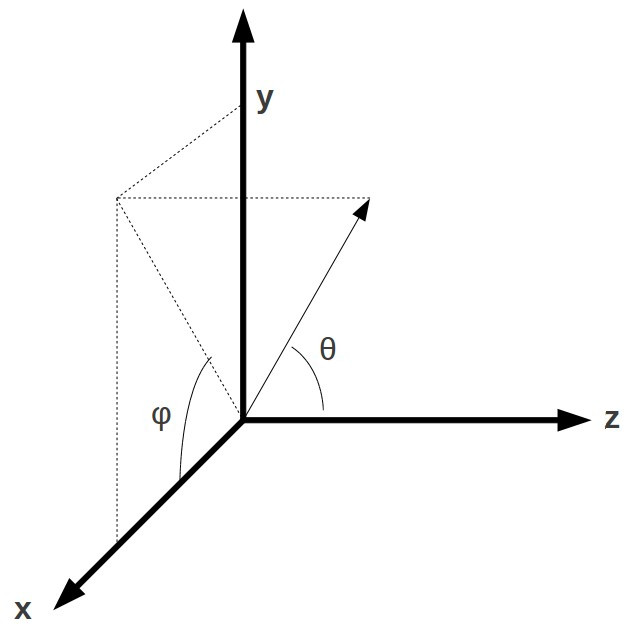
\includegraphics[width=.3\textwidth]{figures/CMS_CoordSys.jpg}
  \caption{CMS coordinate system.}
  \label{fig:CMS_CoordSys}
\end{figure}

\subsection{The magnet}
The CMS superconducting magnet is an hollow cylinder (13 m long, 6 m of diameter, showed in fig.~\ref{fig:CMS_solenoid}). In the niobium and titanium fibers that constitute the solenoid, an electrical current of 19 kA flows, providing a maximum magnetic field of 3.8 T and storing a maximum energy of 2.6 GJ. Superconductiong conditions are allowed by a liquid helium cooling system, keeping the solenoid at 4.5 K. In order to avoid stray fields, the magnetic field lines are closed by the return yoke, composed by 10 ktons of magnetized iron blocks, located in the outer part of CMS and alternated to the muon chambers. The homogeneus magnetic field inside the detector bends the trajectories of the charged particles, allowing the measurement of their momenta $p$, given the relation with the magnetic field strenght $B$ and the radial coordinate $R$ of the trajectory:
\begin{equation}
p [\text{GeV}] = 0.3 \times B [\text{T}] \times R [\text{m}]. 
\end{equation}

\begin{figure}[!htb]
  \centering
    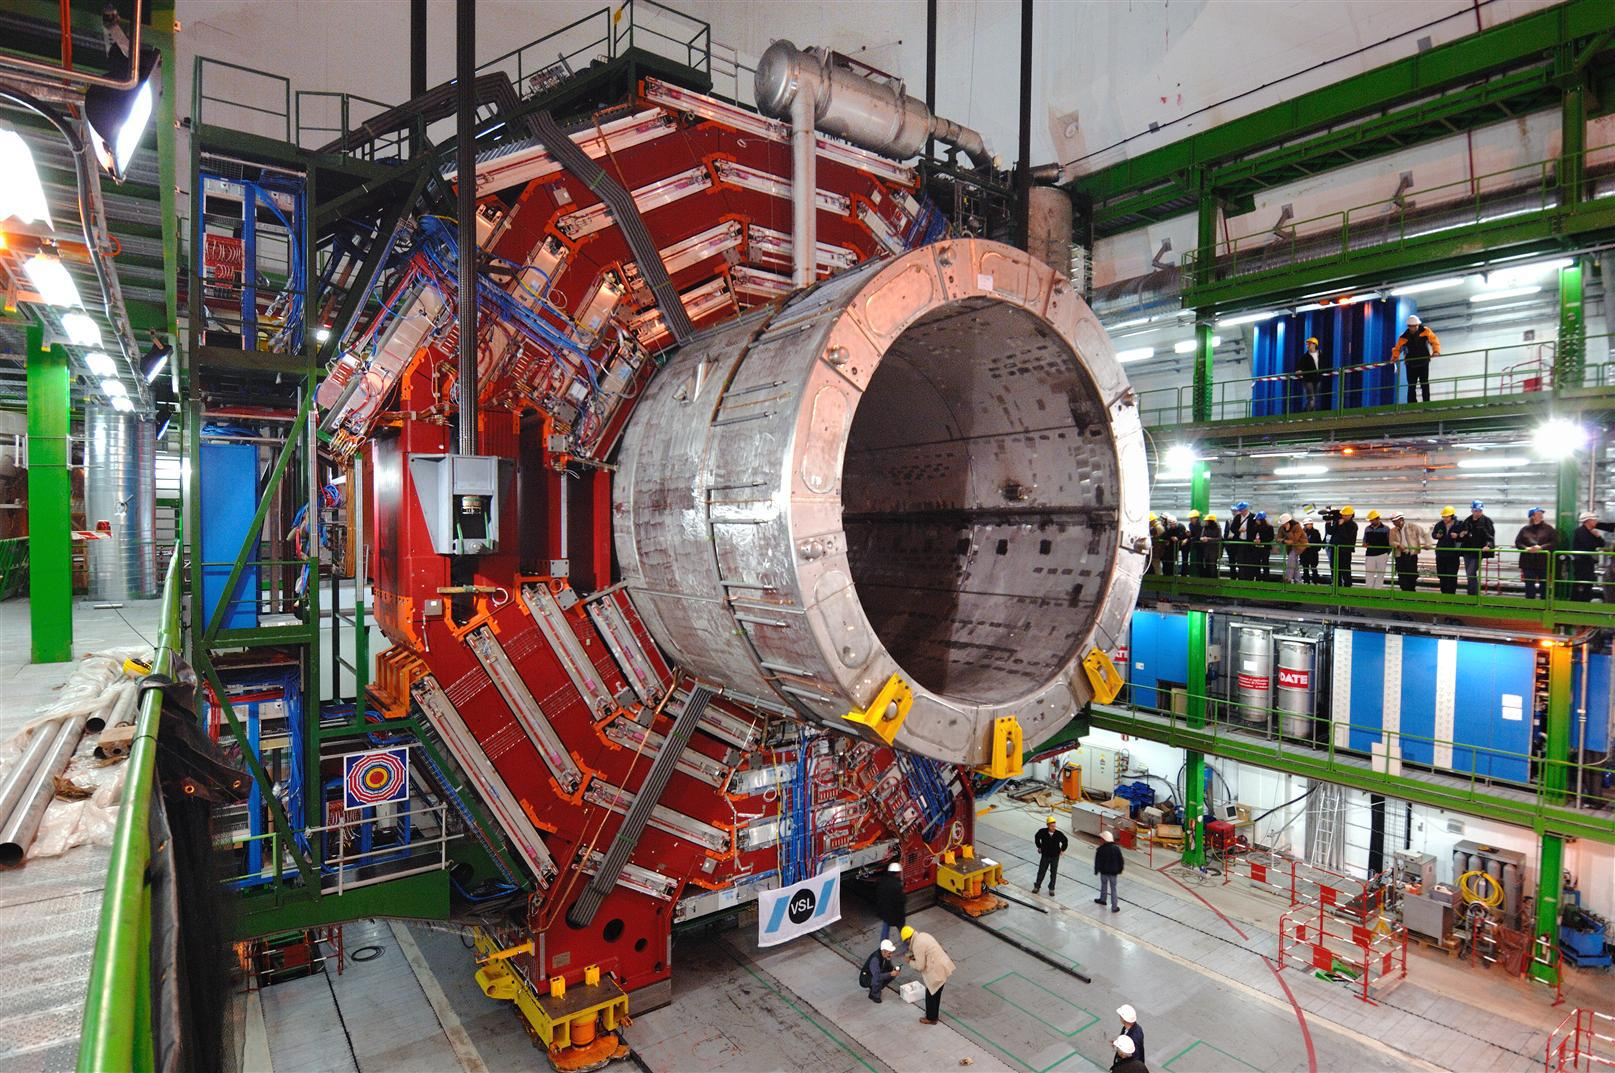
\includegraphics[width=.5\textwidth]{figures/CMS_solenoid.jpeg}
  \caption{Installation of the superconducting solenoid in the CMS cavern.}
  \label{fig:CMS_solenoid}
\end{figure}

\subsection{The tracking system}
\begin{figure}[!htb]
  \centering
    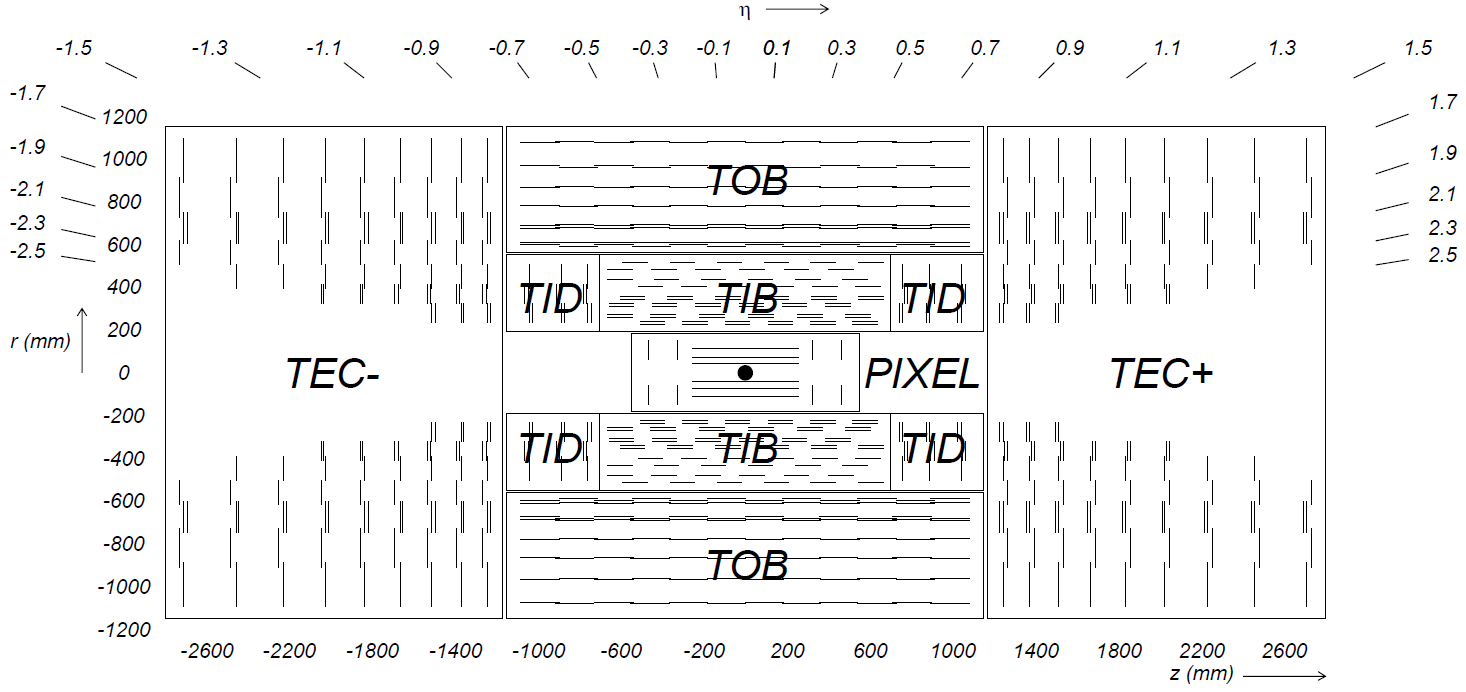
\includegraphics[width=.9\textwidth]{figures/cmstracker.png}
  \caption{The CMS tracking system: the inner pixel detector, close to the interaction point, and the outer strip detector.}
  \label{fig:CMS_tracker}
\end{figure}

The CMS tracking system is composed by a cylinder of silicon detectors (2.5 m of diameter and 5.8 m length). Their design allows a precise reconstruction of the tracks left by charged particles and of the interaction vertices, a fundamental tool to identify heavy quarks (charm, beauty) and leptons (taus).
Tracker detectors cover a pseudorapidity region of $|\eta|<2.5$ and have an active area of $210\text{ m}^2$. The two sub-detectors of the tracking system are the pixel detector, closer to the interaction point, and the strip detector, covering a radius of 0.2 -- 1.2 m. The high granularity of the pixels and micro strips allows to keep the occupancy at acceptable levels, given the high multiplicity of the tracks ($\sim$1 MHz/$\text{mm}^2$). The silicon detectors and the electronic cables are cooled down to a temperature of $\sim 10^{\circ}$ C. The structure of the tracking system is showed in fig.~\ref{fig:CMS_tracker}.

\subsubsection{The pixel detector}
The pixel detector is composed by 66 millions of silicon cells, whose dimensions are $100 \times 150 \text{ }{\mu{m}}^2$, 285 $\mu$m of thickness, placed in 1440 modules. Silicon cells are set in three layers in the barrel region and in two disks at each endcap. Barrel modules are disposed parallel to the magnetic filed, whilst at the endcap they are tilted by about $20^{\circ}$. 
%Il pixel detector \`e costituito da tre strati di rivelatori nel barrel e da due dischi agli endcaps. I moduli nel barrel sono disposti parallelamente al campo magnetico, mentre agli endcaps sono inclinati di circa $20^{\circ}$: le coppie elettrone-lacuna prodotte nel semiconduttore sono allora soggette ad una forza di Lorentz e il loro moto di deriva non avviene pi\`u lungo le linee del campo elettrico, bens\`i esse si sparpagliano lungo diversi pixel. Calcolando il centro della distribuzione di carica raccolta, \`e possibile determinare la posizione della particella carica che ha attraversato il rivelatore con una risoluzione di 15 $\mu$m, sia nel piano $\mathrm{r}\Phi$, sia lungo $\mathrm{z}$.\\
Pixels allow a spatial resolution of 10 $\mu$m in the transverse plane, and of $\sim$20 $\mu$m along the longitudinal coordinate. Their reduced size guarantees an occupancy of $10^{-4}$ per pixel at each bunch crossing, in high luminosity regime.

\subsubsection{The strip detector}
The strip system is divided in the four-layered tracker inner barrel (TIB), covering a region $20 < r < 55$ cm with respect to the interaction point, the six-layered tracker outer barrel (TOB), located at $55 < r < 110$ cm, the three tracker inner disks (TID) and the nine tracker endcaps (TEC) at each cylinder base. Given the lower radiation level at higher radii (and hence a lower occupancy, around few percent), micro strips are bigger than the pixels. Silicon strips in TIB and TID are 320 $\mu$m thick, 10 cm long, and with a pitch ranging from 80 to 120 $\mu$m; strips in TOB and TEC are 25 cm long, with a different thickness (320 $\mu$m for TID, 500 $\mu$m for TEC) and pitch (97-184 $\mu$m). There are 15148 strip modules, and 9.3 million redout channels. The strip spatial resolution is about 20 -- 50 $\mu$m in the transverse plane and about 200 -- 500 $\mu$m along the longitudinal coordinate.
%Nel capitolo 4 descriver\`o le tecniche di ricostruzione delle tracce nei rivelatori al silicio, in particolare dei muoni.\\
%L'efficienza di ricostruzione delle tracce dei muoni \`e stata misurata essere attorno al 99\%, essa cala drasticamente per $|\eta|>2.1$ a causa della ridotta copertura geometrica del pixel detector. Le efficienze di rivelazione degli adroni sono tipicamente pi\`u basse perch\'e interagiscono con il materiale. La risoluzione in $p_T$, sempre per i muoni, \`e attorno all'1-2\% per $|\eta|>1.6$ e per momenti elevati; a momenti pi\`u bassi dominano effetti di scattering multiplo e dipendono dalla quantit\`a di materiale attraversato.\\

\subsection{The elctromagnetic calorimeter}
The CMS electromagnetic calorimeter (ECAL, shown in fig.~\ref{fig:CMS_ecal}) is a homogeneous detector composed by lead tungstate ($\text{PbWO}_4$) scintillating crystals, designed to measure the energy deposits of photons and electrons through their electromagnetic showers. $\text{PbWO}_4$ is transparent and dense (8.3 gr/$\text{cm}^3$); it has a fast time response (the 85\% of the scintillating light is emitted at every bunch crossing, namely 24 ns), high scintillating efficiency and radiation resistance; it has a radiation length is $X_0 = 0.89$ cm and a Moli\`ere radius of 2.19 cm. The ECAL is divided in the barrel region ($\eta < 1.479$, at a radius of 1.3 m) and the endcaps ($1.479 < \eta < 3$).  The 61200 crystals employed in the barrel region, whose size is $(22 \times 22) \text{ mm}^2 \times 23 \text{ cm}$, have a radiation length of $25.8 X_0$; the 7324 crystals in the endcaps, $ 28.6 \times 28.6 \text{ mm}^2 \times 22 \text{ cm}$, have a radiation length of $24.7 X_0$. Before the endcaps, on each side, a pre-shower detector is installed: it is composed by two disks of lead absorber and two layers of silicon strips, up to a radiation length of $3X_0$. It has been designed to distinguish the photons coming from the $\pi^0$ decay from the rare Higgs decay $H \rightarrow \gamma \gamma$. The readout and amplification of the scintillating light, performed by avalanche photodiodes in the barrel and by vacuum phototriodes in the endcaps, requires a stable temperature of $18^{\circ}$ C, mantained by a water cooling system.

\begin{figure}[!htb]
  \centering
    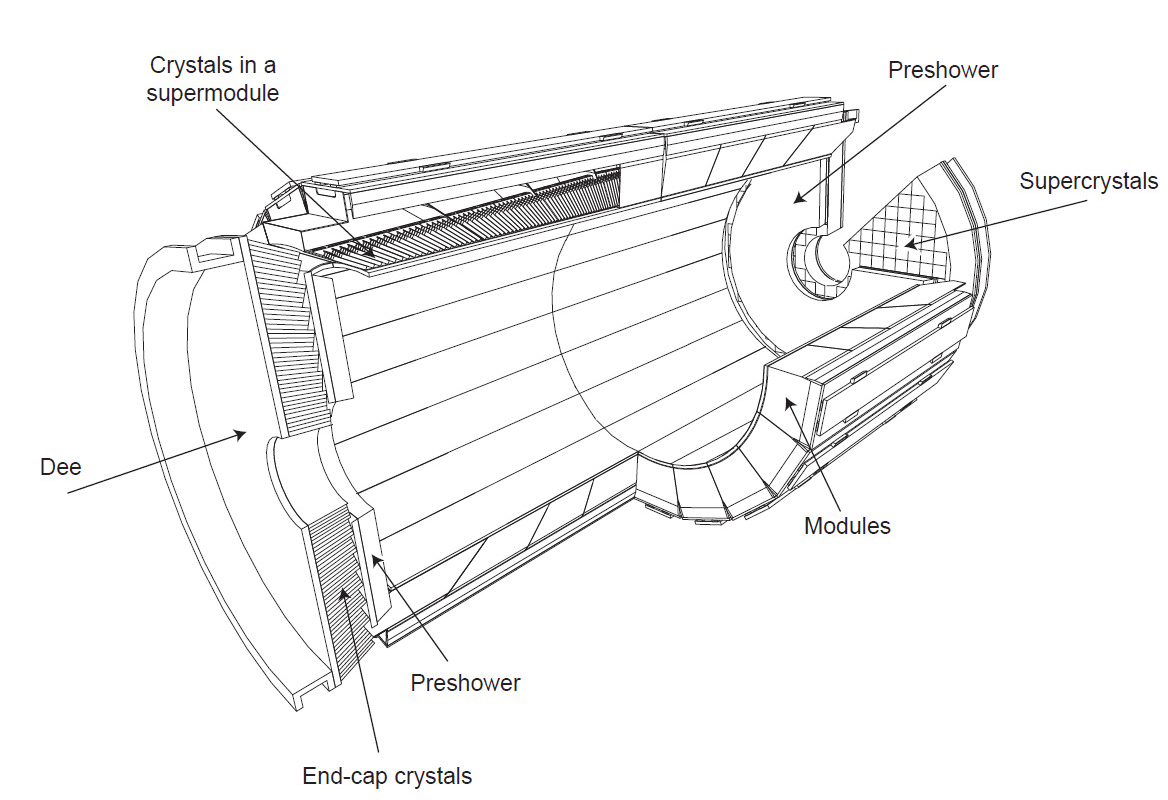
\includegraphics[width=.7\textwidth]{figures/cmsecal.png}
  \caption{The CMS electromagnetic calorimeter.}
  \label{fig:CMS_ecal}
\end{figure}

%\begin{figure}%{l}{0.5\textwidth}
%\centering
%%\includegraphics[scale=0.3]{risoluzione_ECAL.png}
%\caption{Risoluzione in energia di ECAL in funzione dell'energia del fascio di elettroni utilizzato per le misure. Sono mostrati anche i valori per i parametri di fit[16].}
%\label{fig:risoluzione_ECAL}
%\end{figure}

\noindent The energy resolution of the calorimeter is parametrized as:
\begin{equation}
{\left( \frac{\sigma}{E} \right)}^2 = {\left( \frac{S}{\sqrt{E}} \right)}^2 + {\left( \frac{N}{E} \right)}^2 + C^2,
\end{equation}
where $S=0.028 \text{ GeV}^{\frac{1}{2}}$ is the stochastic term, $N=0.12$ GeV is related to noise contribution, and $C=0.003$ is a constant term depending on the calibration.
%In figura \ref{fig:risoluzione_ECAL} sono mostrati i risultati ottenuti da misure di prova con un fascio di elettroni: le stime ottenute sono $S=0.028 \mbox{ GeV}^{\frac{1}{2}}$, $N=0.12 GeV$, $C=0.003$.


\subsection{The hadronic calorimeter}
The hadronic calorimeter (HCAL, displayed in fig.~\ref{fig:CMS_hcal}) is a sampling calorimeter, composed by brass and plastic scintillator layers. It has been designed in order to guarantee a good hermeticity, allowing to perform a precise measurement of the missing transverse energy. It is located within the electromagnetic calorimeter and the solenoid, covering a region of $|\eta|<1.3$ in the barrel, and $1.3<|\eta|<3$ in the endcaps. Brass is non-magnetic and has short interaction length (16.4 cm): the 60 mm thick absorber layers used in the barrel allow to reach 5.6 interaction lengths at $\eta=0$ and 10.8 interaction lenghts at $\eta = 1.3$; the 80 mm thick layers in the endcaps reach 11 interaction lenghts. An additional calorimetric layer has been installed out of the solenoid, in order to reach 11.8 interaction lenghts in the barrel region. The scintillation light, typically in the blue-violet region of the electromagnetic spectrum, is collected by wavalenght-shifter fibers, translated and amplified by multi-channel hybrid photodiodes, proportionally to the magnitude of the energy deposits. An additional hadronic calorimeter has been placed in the forward region, $3 < |\eta| < 5.2$, at 11.2 m from the interaction point. It has beeen designed to afford the high levels of radiations: it is composed by 55 mm thick absorber layers of stainless-steel, and quartz fibers, able to detect the Cherenkov scintillating light of the charged particles of the hadronic showering. A longitudinally segmentation allow to distinguish hadronic particles from electromagnetic components.
The energy resolution of the hadronic calorimeter is:
\begin{equation}
\left( \frac{\sigma}{E} \right) \approx \frac{a}{\sqrt{E}} \oplus b\%,
\end{equation}
where $a=65\%$ in the barrel region, $85\%$ in the endcaps, $100\%$ in the forward region, and $b=5\%$.

\begin{figure}[!htb]
  \centering
    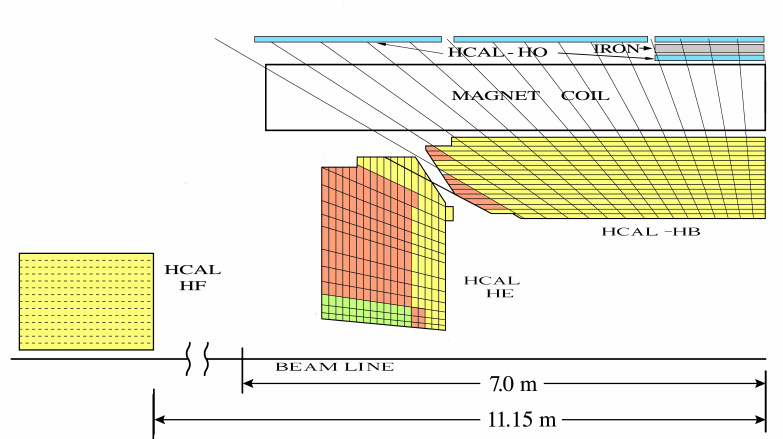
\includegraphics[width=.7\textwidth]{figures/cmshcal.png}
  \caption{The CMS hadronic calorimeter.}
  \label{fig:CMS_hcal}
\end{figure}


\subsection{The muon system}


The outer system of the CMS experiment consists into gas detectors for identifying muons, that are located between the iron return yokes, designed to close the magnetic field generated by the solenoid. In the barrel region, where a smaller number of muons is expected and the magnetic field is less strong, Drift Tubes (DT) detectors are installed. In the endcaps, where the flux of particles is larger, Cathod Strip Chambers (CSC) are used, and disposed in three disks. CSCs are designed to allow faster responses, higher granulatiy and radiation resistance. Resistive Plate Chambers (RPC) are installed both in the barrel and in the endcaps as additional triggering system. The geometry of the muon system is showed in fig.~\ref{fig:CMS_muon}; it consists of 250 DTs, 530 CSCs, 610 RPCs, and it covers a region $|\eta|<2.4$.

\begin{figure}[!htb]
  \centering
    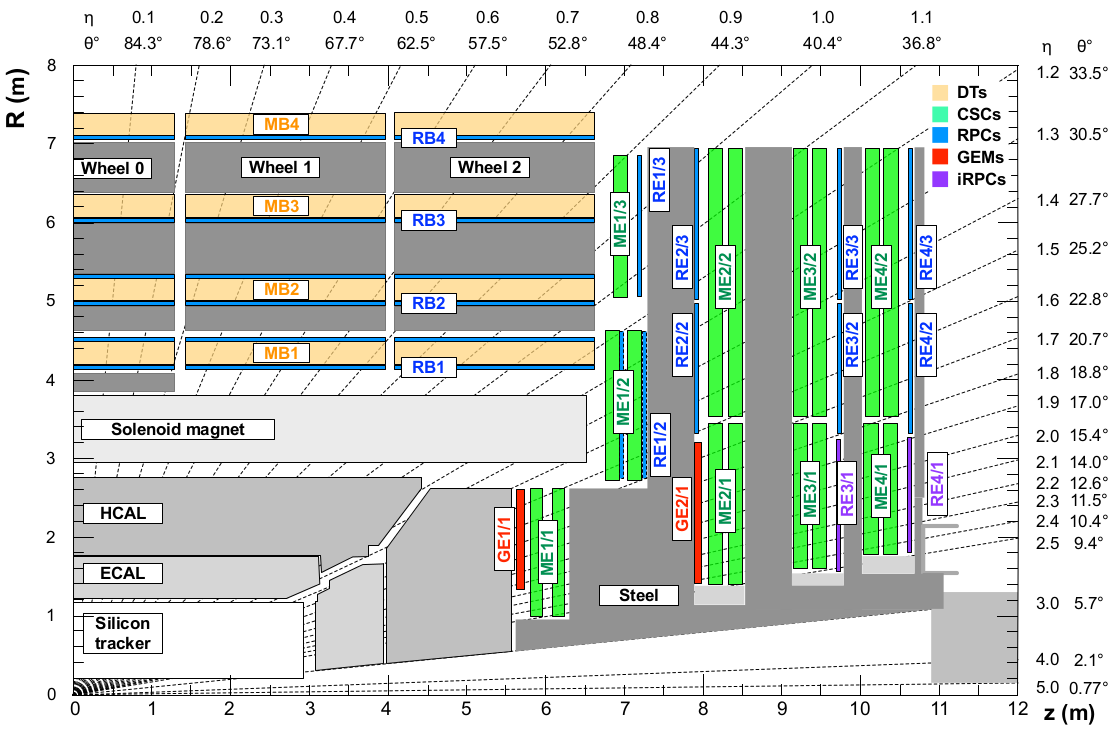
\includegraphics[width=.9\textwidth]{figures/cmsmuon.png}
  \caption{Section of CMS detector, in the plane $\mathrm{rz}$, parallel to the beamline, that emphasizes the location of the muon detectors, in particular: Drift Tubes (DT, in yellow); Cathode Strip Chambers (CSC, in green); Resistive Plate Chambers (RPC, in blue).}
  \label{fig:CMS_muon}
\end{figure}


\subsubsection{The Drift Tubes}
Drift Tube detectors cover a region of $|\eta|<1.2$ and are arranged in four stations, segmented along the beam line in five wheels. The basic element of the detector is the cell, that has a size $42 \times 13 \text{ mm}^2$. Each cell is filled with a gas mixture (85\% argon, 15\% $\text{CO}_2$), in which the process of ionization takes places; the ionization electrons drift from the 50 $\mu$m thick steel anodic wire, in the center of the cell, towards the aluminium cathodic strips, located at its edge. Additional electrodes on the surface of the cells allows to shape the electric field, in order to make the drift speed of the electrons uniform: the muon position is then extrapolated from the measurement of the drift time. Every station is composed by three cells superlayers. In the inner and the outer superlayers, the cells are oriented such in a way that the anodic wire is located along the $z$ axis, in order to measure the $\phi$ coordinate. In the intermediate superlayer, wires are parallel to the radial coordinate, hence they can measure the $z$ position. The spatial resolution of the system is 100 $\mu$m in the $r \phi$ plane, 1 mrad in the $\phi$ coordinate, and 150 $\mu$m in the longitudinal $z$ coordinate.

\subsubsection{The Cathode Strip Chambers}
Cathode Strip Chambers cover a region of $0.9<|\eta|<2.4$, overlapping with the DT in the pseudorapidity range $0.9 < |\eta| < 1.2$. The anodic wires inside each CSC are located into six planes, with the aim of measuring the radial coordinate; the wire planes are perpendicularly crossed by cathodic strips, disposed along the radial direction to measure the $\phi$ coordinate. Ionization electrons produced by muons passing through the gas mixture in the chambers migrate towards the anode, inducing a charge distribution on the cathodes, from which the azimuthal coordinate can be reconstructed. The spatial resolution in the $r$ coordinate is 200 $\mu$m, and it is 75 -- 150 $\mu$m in the $r \phi$ plane. CSCs are arranged in four disks and in three concentric rings.

\subsubsection{The Resistive Plate Chambers}
Resistive Plate Chambers (RPC) are located both in the barrel (disposed in six layers) and in the endcap region (three layers), up to a pseudorapidity of $|\eta|<1.6$. These gas detectors are charged at very high voltages, in order to work in the avalanche ionization mode. The plastic resitive plates are equipped with readout strips. The spatial resolution of the detector is low (1-2 cm), but the fast timing response (2-3 ns) and good time resolution (1 ns) allow to employ RPCs as an additional triggering system and to profit of a precise measurement of the bunch-crossing time.

%\subsection{Other CMS sub-detectors}
%Tracciatori e camere per i muoni coprono una regione di $|\eta|<2.5$, gli apparati calorimetrici arrivano fino ad $|\eta|<5.2$. Ci sono altri due rivelatori che permettono misure nella regione $5 \leq |\eta| \leq 11$, TOTEM e CASTOR. TOTEM sfrutta dei rivelatori a gas per le misure di scattering elastico protone protone in funzione del loro momento. CASTOR \`e un calorimetro elettromagnetico ed adronico che raccoglie luce Cherenkov, serve per misure di QCD in collisioni p-p, p-ione, ione-ione.

\subsection{The trigger system and data acquisition}
The CMS trigger system has been designed considering the high instantaneous luminosity, such that it can provide a fast response and it allows to reduce the nominal event rate of 40 MHz in proton proton collision. The complexity of the CMS detector and the very high number of readout channels result into a huge amount of data per event, approaching the order of few MB per bunch crossing, hence 40 TB per second. The handling and the recording of data is currently limited at the order of $\sim$100 Hz; hence, applying online selections to skim the events that are going to be written on tape, without rejecting interesting signals of hard processes and rare phenomena becomes a crucial and challenging point for every data analysis. Events are filtered by trigger selections at different levels: the Level-1 (L1) trigger is an hardware device, that allows to reduce the event rate from 40 MHz to the order of 100 kHz; the High Level Trigger (HLT) is a set of software algorithms that skims the event rate down to few hundred Hz. Once the trigger decisions are taken, the final events are handled by the Data Acquisition System (DAQ), that collects the informations coming from to the subdetectors and sends them to the storage devices.

\subsubsection{The Level-1 trigger}
The L1 trigger is an hardware device composed by customized electronics, and it accesses the informations coming from the calorimeters and the muon system, while the tracker is not considered given the excessively large bandwidth needed by its readout channels. The L1 trigger perform a first raw local reconstruction of each object, called ``trigger primitive''. The L1 trigger is composed by three subsystems: the calorimeter trigger, the muon trigger (divided in three independent sub-subsystems for each muon subdetector, namely DTs, RPCs and CSCs), and the global trigger, that combines the informations of the former subsystems. The best quality trigger primitives reconstructed by the calorimeter and muon detectors (namely, roughly reconstructed electrons, photons, muons, jets, jets coming from the hadronic decays of tau leptons, and missing energy) are handled by the global trigger, who takes the decision of discarding or keeping the event every 3.2 $\mu$s. The simplest trigger selections require the presence of a single object, whose energy or transverse momentum is higher than a certain threshold; more complicated triggers involve multiple objects or geometrical selections, that can be performed in parallel up to 128 simultaneous requirements.

\subsubsection{The High Level Trigger}
The HLT skims the L1 output rate down to few hundreds of Hz by applying a set of algorithms implemented in the same software used for the offline analysis, consisting in the event reconstructions exploiting the whole informations coming from all subdetectors. The computing time is still a crucial factor, hence selections applied to HLT physics objects are generally less accurate than those of the offline analysis; furthermore, HLT can discard the event even before its full reconstruction (\textit{i.e.} by looking only at certain region of the detectors). Events filtered by the HLT decisions are assigned to precise trigger paths and recorded in precise categories of datasets.

\subsubsection{Data acquisition, computing and storage}
The DAQ system deals with the storage, transfer and handling of the data collected by CMS; it also supports and stores the data simulations and calibrations of the subdetectors. The CMS computational resources are located in worldwide distributed data nodes, called Tiers. The CMS software (CMSSW) is based on an object oriented architecture (mainly C++). The basic unity of every data, both real and simulated ones, is the Event, that could contain very rough informations (RAW data format) or higher level refined objects (AOD, Analysis Object Data) where all the calibrations and corrections needed to properly deal with the final physics objects are already in place. Data are handled by C++ or python modules, and the outputs are written in ROOT files. [citazione]

\subsection{Particle Flow event reconstruction}
-- ref from paper
The global event reconstruction at CMS relies on the particle flow (PF) [69, 70] algorithm, which
reconstructs and identifies each individual particle with an optimized combination of informa-
tion from the various elements of the CMS detector. The energy of photons is directly obtained
from the ECAL measurement, while the energy of electrons is determined from a combina-
tion of the electron momentum at the primary interaction vertex as determined by the tracker,
the energy of the corresponding ECAL cluster, and the energy sum of all bremsstrahlung pho-
tons spatially compatible with originating from the electron track. The momentum of muons
is obtained from the curvature of the corresponding track. The energy of charged hadrons is
determined from a combination of their momentum measured in the tracker and the match-
ing ECAL and HCAL energy deposits, and the energy of neutral hadrons is obtained from the
corresponding ECAL and HCAL energy.
The core of the particle flow reconstruction technique is the algorithm used to link the signals
of the individual subdetectors. The association criteria is purely geometrical. The aim is a
full reconstruction of each single particle, while reducing any possible double counting from
different detectors. Given the granularity of the calorimeters, energy deposits and tracks are
linked if their trajectory intersects one of the calorimetric cells, and likewise clusters in the
ECAL pre-shower, ECAL and HCAL are linked if the cluster position is compatible in the η, φ
plane between the extrapolated track position and the cluster position.


The particle-flow event reconstruction aims at reconstructing and identifying all sta-
ble particles in the event, i.e. electrons, muons, photons, charged hadrons and neu-
tral hadrons, by mean of an optimized combination of informations from all CMS sub-
detectors. The algorithm is described in detail in References [44–46] where information
on its commissioning with early data are also provided. The CMS PF algorithm relies
on a efficient and pure track reconstruction, on a clustering algorithm able to disentangle
overlapping showers, and on an efficient link procedure to connect together the deposits
of each particle in the sub-detectors. Tracks are extrapolated through the calorimeters: if
they fall within the boundaries of one or several clusters, the clusters are associated to
the track. The set of track and cluster(s) constitute a charged hadron and are not con-
sidered anymore in the rest of the algorithm. The muons are identified beforehand so
that their track does not give rise to a charged hadron. The electrons are more difficult to
deal with. Indeed, due to the frequent Bremsstrahlung photon emission, a specific track
reconstruction (the GSF already discussed in Section 2.2.3.1) is needed as well as a ded-
icated treatment to properly attach the photon clusters to the electron and avoid energy
double counting. Once all the tracks are treated, the remaining clusters result in photons
in case of the electromagnetic calorimeter (ECAL), and in neutral hadrons in the case a
hadron calorimeter (HCAL) cluster is matched to an ECAL cluster. Once all the deposits
of a particle are associated, its nature can be assessed, and the information of the sub-
detectors combined to determine optimally its four-momentum. In case the calibrated
calorimeter energy of the clusters, which is simply a linear combination of the ECAL and
HCAL energy deposits, associated to a track is found to be in excess with respect to the
track momentum at more than one sigma, the excess is attributed to an overlapping neu-
tral particle (photon or hadron), carrying an energy corresponding to the difference of
the two measurements. The resulting list of particles, namely charged hadrons, photons,
neutral hadrons, electrons and muons, is then used to reconstruct the jets, the missing
transverse energy, to reconstruct and identify the τ from their decays products and to
measure the isolation of the particles.
The association used in the linking stage is purely geometrical: tracks are linked to calori-
metric clusters if their trajectory intersects one of the calorimetric cells of the cluster; and
likewise clusters in the ECAL preshower, ECAL and HCAL are linked if the cluster posi-
tion measured in the finer granularity subdetector lies within the envelop of the cluster 
in the coarser granularity subdetector. In order to account for uncertainties from mul-
tiple scattering in the track extrapolation and on the estimated position of the shower
maximum in the calorimeters, a geometrical tolerance of the size of one calorimeter cell
is included when defining links; this tolerance can also account for gaps and cracks in
the calorimeters. By design, the linking algorithm is simple and robust, as it does not
rely on the precise knowledge of the position resolution in each subdetector. Special-
ized algorithms are used for linking tracks to recover bremsstrahlung clusters in the
case of electrons by considering tangents to electron trajectories at the crossing points
with the tracker layers. Blocks of one or more linked objects are then processed to iden-
tify and reconstruct particle candidates. Isolated electrons and muons are selected first,
and reconstructed using the dedicated algorithms developed for them; similarly, non-
isolated tracks which satisfy tight muon identification criteria are immediately identi-
fied as muons. Charged hadrons are identified as tracks in the inner tracker, normally
linked to calorimetric deposits if the particle p T is sufficient for the trajectory to reach the
calorimeters. If the momentum measurements from the track and calorimeter are com-
patible, after accounting for non-linearities and zero suppression effects, the best energy
determination is obtained as a combination of the two. If the track momentum signif-
icantly exceeds the measured calorimetric energy, the particle is identified as muon if
it satisfies very loose muon identification criteria; otherwise, tight track quality require-
ments are applied to to reject mis-reconstructed tracks. If instead an excess of calorimetric
energy deposition is found with respect to the momentum of the associated track, e.g. in
the case of collimated hadronic jets, the residual energy is identified as a photon or a neu-
tral hadron. Additional photons and neutral hadrons are also identified from calorimetric
deposits not linked to any track.
\subsection{Physics objects}

\subsubsection{Track and vertex reconstruction}
\subsubsection{Electron reconstruction}
\subsubsection{Photon reconstruction}
\subsubsection{Muon reconstruction}
L'intero sistema misura in maniera ``standalone'' l'impulso con una risoluzione in $p_T$ di circa $\Delta p_T/p_T \approx 8-15\%$ per muoni di $p_T = 10$ GeV/c e di $\Delta p_T/p_T \approx 20-40\%$ per muoni di $p_T = 1$ TeV/c. Combinando con la misura nei rivelatori al silicio la risoluzione passa rispettivamente all'$1\%$ e al $7-16\%$.\\
\subsubsection{Jet reconstruction}
\subsubsection{Tau reconstruction}
\subsubsection{Missing transverse energy reconstruction}
\subsubsection{b-quark tagging}


\section{ATLAS, ALICE, LHCb detectors}

\subsection{ATLAS}
ATLAS (A Toroidal LHC ApparatuS) is a multi-purpose experiment, that shares the same scientifical aims of CMS. The simultaneous observation of an Higgs boson-like particle at the two experimental facilities represented an irrefutable proof of the discovery of the Higgs boson.\\
ATLAS has a cylindrical shape (diameter of 25 m, length of 46 m) and weights 7000 tons. Like CMS, ATLAS is composed by many sub-detectors: trackers, calorimeters and muon system. The ATLAS magnetic field is provided by a solenoid, located inside the cylinder, and a big toroid, located outside the sub-detectors, able to reach a magnetic field of 2 T at the interaction point. The main differences among the two experiments are listed below.

\begin{itemize}
\item {\itshape Tracker --} the CMS tracker has a better $p_T$ resolution (mainly due to the higher magnetic field): $\sigma_{p_T}/p_T \approx 5 \cdot 10^{-4} p_T + 0.01$ at ATLAS; $\sigma_{p_T}/p_T \approx 1.5 \cdot 10^{-4} p_T + 0.005$ at CMS.
\item {\itshape Electromagnetic calorimeter --} the CMS electromagnetic calorimeter is completely enclosed inside the solenoid, whilst ATLAS calorimeter is outside of the solenoid. The particles going through the solenoid suffer an energy loss and a consequent deterioration of the energy resolution. The CMS ECAL has an enery resolution of $\sigma_E /E \approx 3\%/\sqrt{E}$; the ATLAS calorimeter has a sandwich structure (liquid argon and lead layers) and a resolution of $\sigma_E / E \approx 10\%/\sqrt{E}$.
\item {\itshape Hadronic calorimeter --} the CMS HCAL is partly inside the solenoid, partly outside, depauperating the resolution. The ATLAS hadronic calorimeter (made of iron and plastic scintillator tiles) has an energy resolution $\sigma_E /E \approx 50\%/\sqrt{E} + 0.03$ GeV; CMS HCAL has a resolution of $\sigma_E /E \approx 100\%/\sqrt{E} + 0.05$ GeV.
\item {\itshape Muon system --} the peculiar geometry of the ATLAS muon system allows a better resolution of the standalone measurement of the muon momenta (\textit{i.e.}, without using tracker and calorimeters), that is around 10\% at 1 TeV. CMS has better performance when combining the informations coming from the inner detectors (7\% at 1 TeV against the 35\% for the standalone measurement).
\end{itemize}

\subsection{ALICE}
ALICE (A Large Ion Collider Experiment) studies the heavy ion collisions (lead-lead) or proton-ion in order to explore the physics of the hadrons in high density (or temperature) regimes, when a new state of matter appears, the so-called quark-gluon plasma (QGP). The QGP played a crucial role in the very first instants of life of the universe.

\subsection{LHCb}
LHCb (Large Hadron Collider beauty) is a detector designed to study the b quark properties, in particular the CP violation and other rare phenomena involved in b hadrons. The final aim of these measurements is trying to solve the matter-antimatter asymmetry problem.

\vspace*{1\baselineskip}

\noindent The three detectors are depicted in fig.~\ref{fig:ATLAS}--\ref{fig:LHCb}.


\begin{figure}%{l}{0.5\textwidth}
\centering
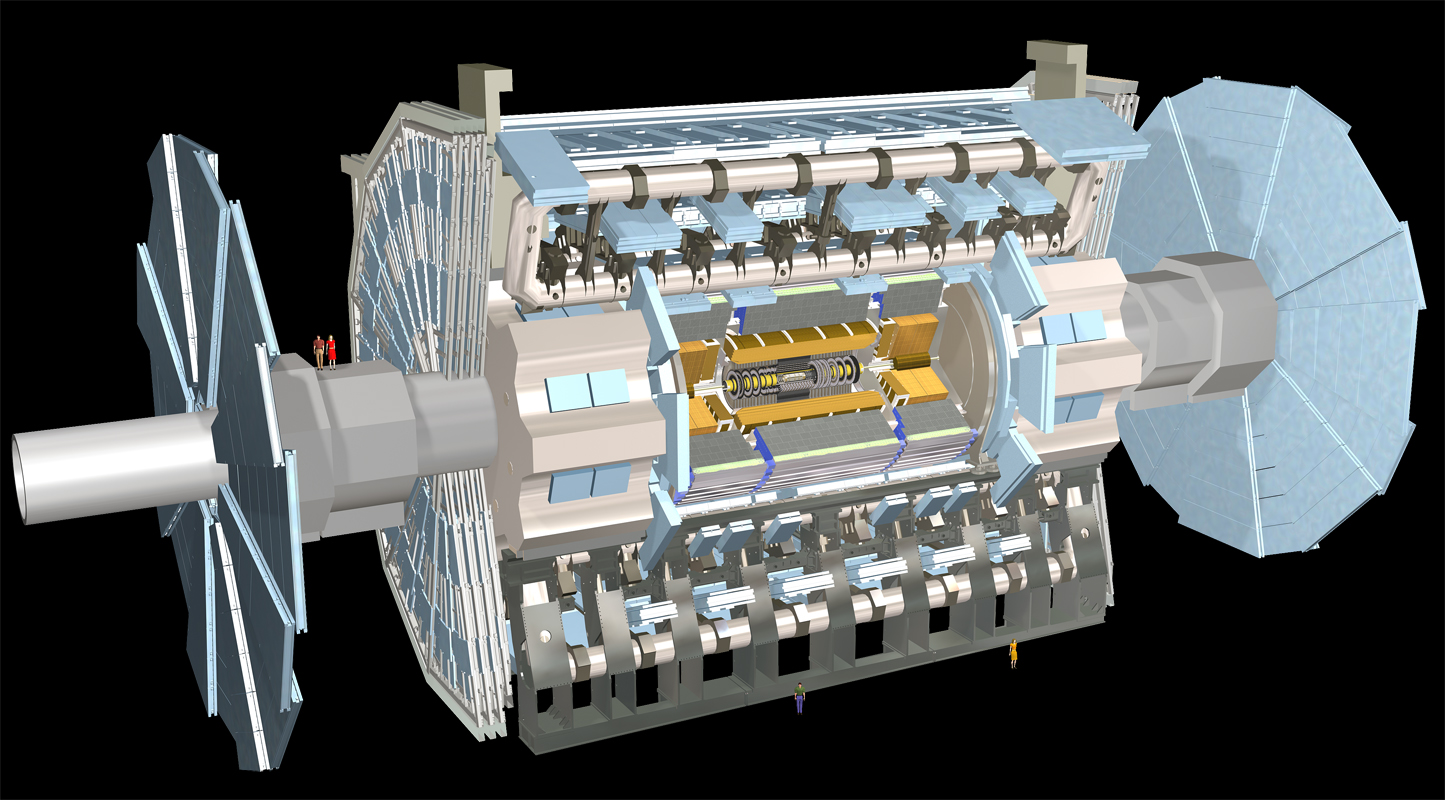
\includegraphics[width=.6\textwidth]{figures/ATLAS.jpg}
\caption{The ATLAS experiment.}
\label{fig:ATLAS}
\end{figure}

\begin{figure}%{l}{0.5\textwidth}
\centering
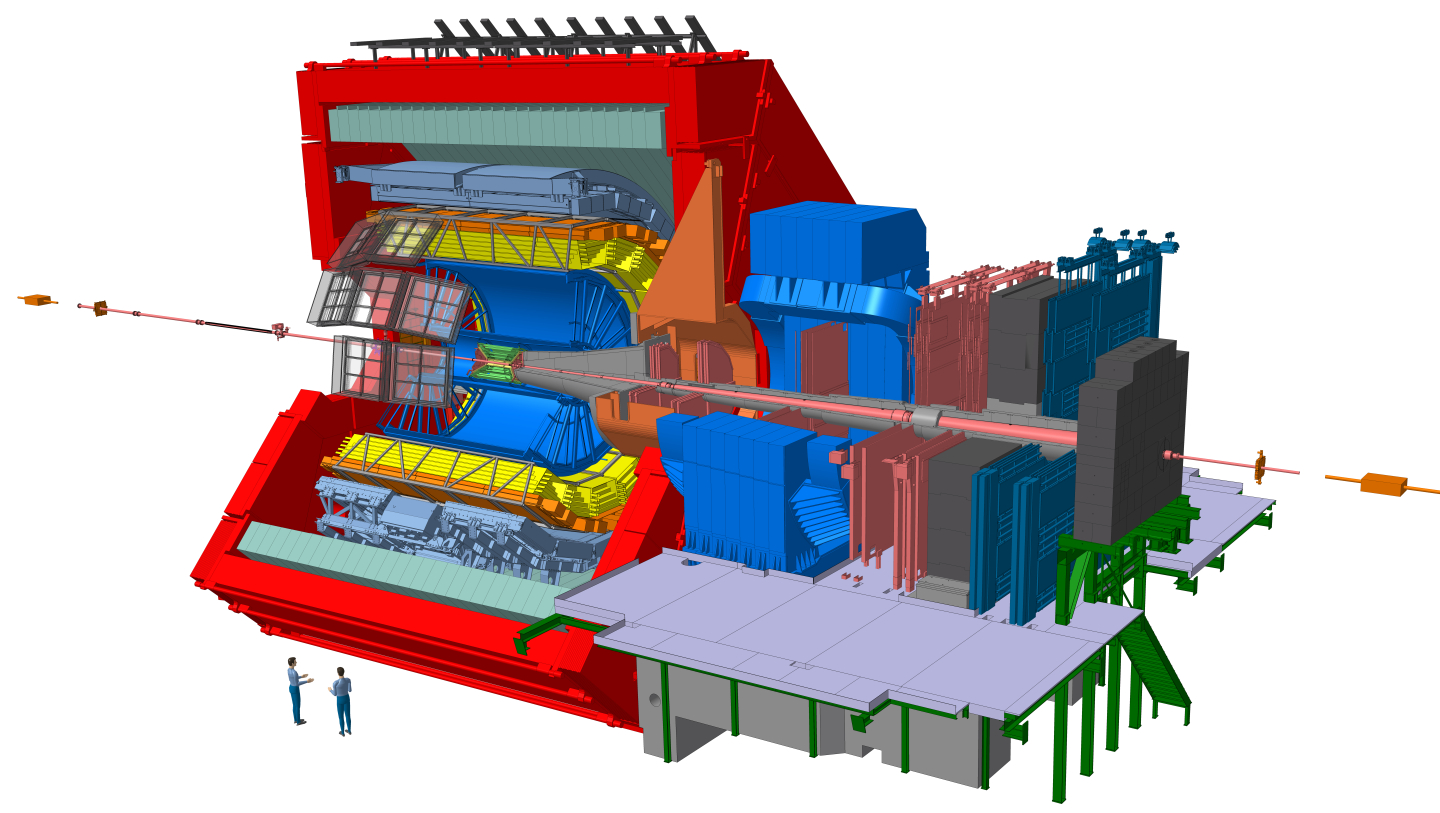
\includegraphics[width=.6\textwidth]{figures/ALICE.jpg}
\caption{The ALICE experiment.}
\label{fig:ALICE}
\end{figure}

\begin{figure}%{l}{0.5\textwidth}
\centering
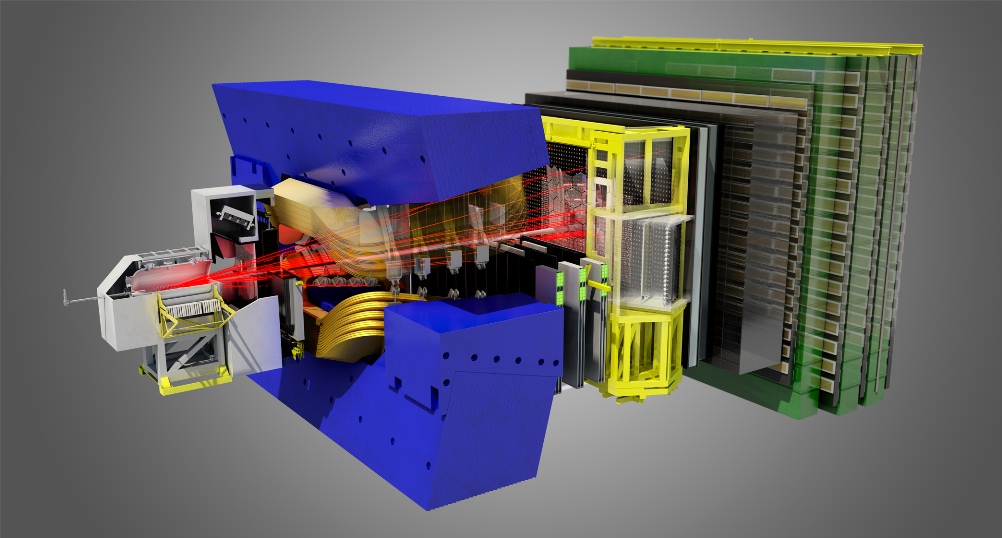
\includegraphics[width=.6\textwidth]{figures/LHCb.png}
\caption{The LHCb experiment.}
\label{fig:LHCb}
\end{figure}

\clearpage
